\documentclass[a4paper,11pt]{article}

\usepackage[utf8]{inputenc}
\usepackage[T1]{fontenc} % LY1 also works

%% Font settings suggested by fbb documentation.
\usepackage{textcomp} % to get the right copyright, etc.
\usepackage[lining,tabular]{fbb} % so math uses tabular lining figures
\usepackage[scaled=.95,type1]{cabin} % sans serif in style of Gill Sans
\usepackage[varqu,varl]{zi4}% inconsolata typewriter
\useosf % change normal text to use proportional oldstyle figures
%\usetosf would provide tabular oldstyle figures in text

\usepackage{booktabs}
\usepackage{microtype}
\usepackage{comment}
%\usepackage{hyphenat}

\renewcommand{\d}{\mathrm{d}}
\renewcommand{\a}{\mathrm{a}}
\newcommand{\orb}{\mathrm{orb}}
\newcommand{\cm}{\mathrm{cm}}
\newcommand{\CE}{\mathrm{CE}}
\newcommand{\TCE}{\mathrm{TCE}}
\newcommand{\spin}{\mathrm{spin}}
\newcommand{\bind}{\mathrm{bind}}
\newcommand{\init}{\mathrm{init}}
\newcommand{\fin}{\mathrm{fin}}
\newcommand{\age}{\mathrm{age}}
\newcommand{\MS}{\mathrm{MS}}
\newcommand{\BGB}{\mathrm{BGB}}
\newcommand{\MT}{\mathrm{MT}}
\newcommand{\WA}{\mathrm{WA}}
\newcommand{\comp}{\mathrm{comp}}
\newcommand{\wind}{\mathrm{wind}}
\newcommand{\kick}{\mathrm{kick}}
\newcommand{\BH}{\mathrm{BH}}
\newcommand{\NS}{\mathrm{NS}}
\newcommand{\remnant}{\mathrm{remnant}}
\newcommand{\prog}{\mathrm{prog}}
\newcommand{\CO}{\mathrm{CO}}


\newcommand{\md}{m_\mathrm{d}}
\newcommand{\ma}{m_\mathrm{a}}
\newcommand{\rAd}{\ve{r}_{\mathrm{A}_\mathrm{d}}}
\newcommand{\Ad}{{\mathrm{A}_\mathrm{d}}}
\newcommand{\Aa}{{\mathrm{A}_\mathrm{a}}}
\newcommand{\XAd}{X_{\mathrm{A}_\mathrm{d}}}
\newcommand{\XL}{X_{\mathrm{L}}}
\newcommand{\XLz}{X_{\mathrm{L,0}}}
\newcommand{\urAd}{\hat{\ve{r}}_{\mathrm{A}_\mathrm{d}}}
\newcommand{\rAa}{\ve{r}_{\mathrm{A}_\mathrm{a}}}
\newcommand{\rA}{\ve{r}_{\mathrm{A}}}
\newcommand{\betamt}{\beta_\mathrm{MT}}
\newcommand{\taumt}{\tau_\mathrm{MT}}
\newcommand{\mper}{m_\mathrm{per}}
\newcommand{\qper}{r_\mathrm{p,\,per}}
\newcommand{\eper}{e_\mathrm{per}}
\newcommand{\srel}{\sigma_\mathrm{rel}}
\newcommand{\mint}{M_\mathrm{int}}
\newcommand{\eff}{\mathrm{eff}}


\usepackage{graphicx}
\usepackage{enumitem}
\usepackage{listings}
%\setlist{xleftmargin=0.in}
\lstset{basicstyle=\ttfamily,frame=single,xleftmargin=0em,xrightmargin=0em}
\usepackage[os=win]{menukeys}
\renewmenumacro{\keys}[+]{shadowedroundedkeys}
\usepackage{framed}
\usepackage{etoolbox}
\AtBeginEnvironment{leftbar}{\sffamily\small}

\newcommand{\sse}{\textsc{SSE}}
\newcommand{\bse}{\textsc{BSE}}
\newcommand{\mse}{\textsc{MSE}}

\renewcommand{\S}{Section}
\newcommand{\Ss}{Sections}
\newcommand{\F}{Fig.}
\newcommand{\Fs}{Figs}
\newcommand{\Eq}{Equation}
\newcommand{\Eqs}{Equations}
\newcommand{\eq}{Equation}
\newcommand{\eqs}{Equations}
\newcommand{\code}{Code snippet}

\newcommand{\gconst}{\mathcal{G}}
\newcommand{\msun}{\mathrm{M}_\odot}
\newcommand{\rsun}{\mathrm{R}_\odot}
\newcommand{\lsun}{\mathrm{L}_\odot}
\newcommand{\au}{\textsc{au}}
\newcommand{\kms}{\mathrm{km\,s^{-1}}}
\newcommand{\yr}{\mathrm{yr}}

\renewcommand{\lstlistingname}{Code snippet}

\usepackage[left=3.0cm,top=3.0cm,bottom = 3.0cm,right=3.0cm,nohead]{geometry}
\usetikzlibrary{chains,arrows,shapes,positioning}
\usepackage{hyperref}

\newcommand\AutoCalc{\textsf{AutoratingCalculator}}
%\renewcommand\abstractname{Introduction}

\title{User manual for the Multiple Stellar Evolution (MSE) code}
\author{Adrian Hamers (\url{hamers@mpa-garching.mpg.de})\\\url{https://mse-group.net}}
\date{\url{https://github.com/hamers/mse} \\ September 30, 2020}
\begin{document}
\maketitle

%\begin{abstract}
%\end{abstract}

\tableofcontents
\clearpage

\section{Introduction}
This is the user manual for the Multiple Stellar Evolution (\mse) code. \mse~models the long-term evolution of hierarchical multiple-star systems (binaries, triples, quadruples, and higher-order systems) from the main sequence until  the remnant stages. It takes into account gravitational dynamical evolution, stellar evolution (using the \sse~tracks), and binary interactions (such as mass transfer and common-envelope evolution). It includes routines for external perturbations from flybys in the field, or (to limited extent) encounters in dense stellar systems such as galactic nuclei.


\section{Installation}
\mse~is written primarily in \textsc{C++} but also uses some \textsc{Fortran} routines. A \textsc{Python} interface is included for easy use. The source code is available\footnote{At the moment of writing, the \texttt{GitHub} repository is private. Access will be given on a per-request basis (please contact the author). In the future, the repository will be made public.} at \href{https://github.com/hamers/mse}{https://github.com/hamers/mse} (it is assumed that you have \texttt{git} installed). To download it, you can use the following command:
\begin{lstlisting}[caption={},label={code:wrap},language=bash]
git clone https://github.com/hamers/mse.git
\end{lstlisting}
This will create a new directory \texttt{mse} within your current directory. 

To install (i.e., compile) \mse, \textsc{C++} and \textsc{Fortran} compilers are required, as well as Python (2/3) in order to use the Python interface. A \texttt{Makefile} is included which should be used for compilation. By default, it assumes that \texttt{g++} and \texttt{gfortran} are available on the system. To compile, simply type
\begin{lstlisting}[caption={},label={code:wrap},language=bash]
make
\end{lstlisting}
If \texttt{g++} and/or \texttt{gfortran} are not available, you will need to modify the lines
\begin{lstlisting}[caption={},label={code:wrap},language=bash]
CXX = g++
FC = gfortran
\end{lstlisting}
in the \texttt{Makefile} accordingly to correspond to your \textsc{C++} and \textsc{Fortran} compilers. 

The compilation will typically take a few seconds. If compiled successfully, you should see the message
\begin{lstlisting}[caption={},label={code:wrap},language=bash]
The shared library mse has been created successfully.
\end{lstlisting}

In order to use the \textsc{Python} interface, the \texttt{numpy} package is required. Also, \texttt{Matplotlib} is needed to produce plots in some of the scripts provided with the code.
 
%\begin{leftbar}
%You may also prepare the group list in Excel. List the IDs in column A and the IDs in column B. Save the file as a Comma separated values file (CSV). In the Export Filter Settings, set text delimiter to %blank, and field separator to comma (\texttt{,}).
%\end{leftbar}


%linewidth=20cm

\section{Testing the installation}
To make sure that the code has been properly installed, you can use a \textsc{Python} test script which is included. In the main directory of \mse, simply type
\begin{lstlisting}[caption={},label={code:wrap},language=bash]
python3 test_mse.py
\end{lstlisting}
This will run a number of tests, producing some output. If all tests ran successfully, you should see the message
\begin{lstlisting}[caption={},label={code:wrap},language=bash]
All tests passed!
\end{lstlisting}

\begin{leftbar}
Specific tests (see \texttt{test\_mse.py} for details) can be initiated by passing the ``\texttt{--t X}'' command line argument to \texttt{test\_mse.py}, where \texttt{X} is the number of the test to run. In addition, some tests have a `detailed' mode which is more extensive, but takes significantly longer to run. The detailed mode can be activated by adding the command line argument ``\texttt{--m 1}''.
\end{leftbar}

\section{Code usage -- \textsc{Python}}
\label{sect:usepy}
\mse~can be used with the \textsc{Python} interface (recommended for most users), but also directly within \textsc{C++} (recommended for advanced users only)\footnote{At the moment of writing, \mse~has been most tested with the \textsc{Python} interface. Usage within \textsc{C++} is less tested.}. In this section, we describe usage within \textsc{Python}.

\subsection{Basic}%: using \texttt{run\_system.py} and/or the wrapper function \texttt{evolve\_system()}}
\label{sect:usepy:basic}
\subsubsection{From the command line: \texttt{run\_system.py}}
\label{sect:usepy:basic:run}
The easiest way to run a system in \mse~is by using the included \texttt{run\_system.py} script. This script has the convenience of being accessible fully within the command line. It produces basic plots with the time evolution of some quantities, mobile diagrams, and positions. It currently supports two types of hierarchical configurations: `fully nested' systems, in which the number of levels in the system is maximised, and `2+2 quadruple' systems (see \F~\ref{fig:wrapper}).

\begin{figure}
  \center
  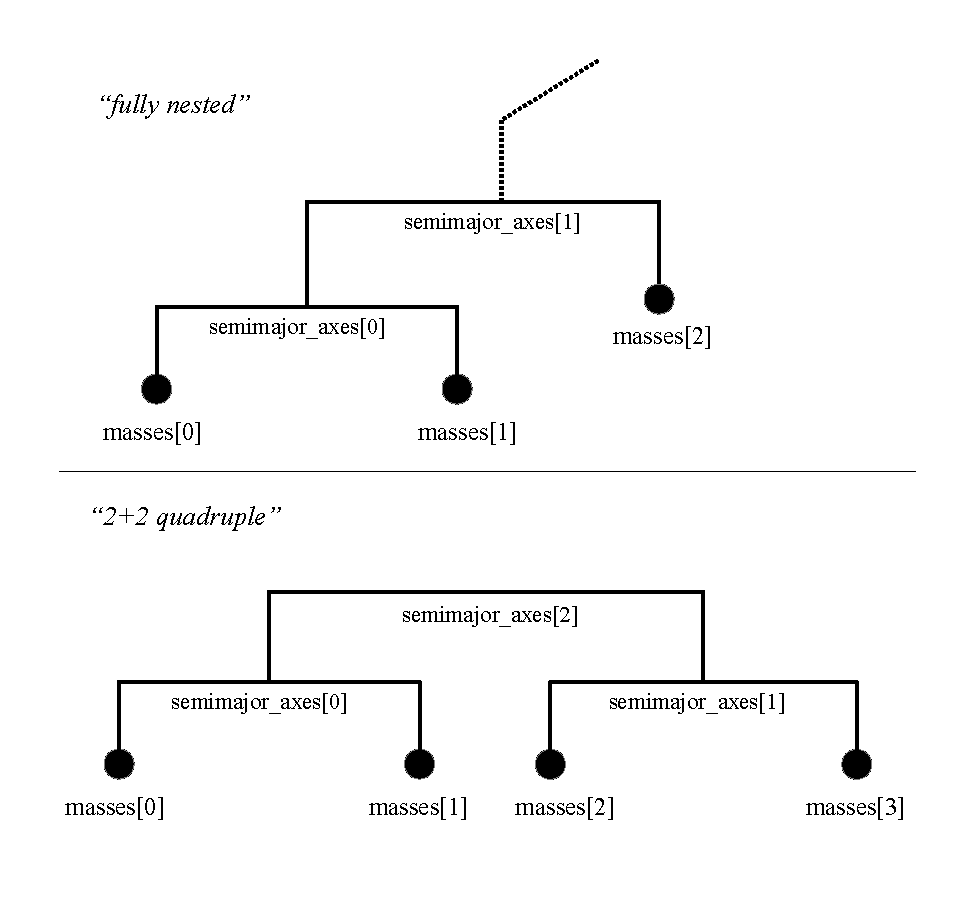
\includegraphics[width=0.65\textwidth,trim=0mm 0mm 0mm 0mm]{figs/wrapper}
  \caption{Illustration of currently supported configurations within the \texttt{run\_system.py} script and the \texttt{evolve\_system()} wrapper function. Also shown are designations within the argument lists (displayed are \texttt{masses} and \texttt{semimajor\_axes}, but the same orders apply to other properties of bodies/orbits). Top: a `fully nested' configuration (explicitly showing the simplest case of a triple). Bottom: a 2+2 quadruple system. }
\label{fig:wrapper}
\end{figure}

For example, a hierarchical triple can be run simply with the following command shown in \code~\ref{code:simpletriple}. 
\begin{lstlisting}[caption={Example usage of \texttt{run\_system.py} for a triple.},label={code:simpletriple},language=bash]
python3 run_system.py --configuration "fully_nested"
--masses 40 10 2 --metallicities 0.02 0.02 0.02 
--smas 15 120 --es 0.1 0.2 --is 0.001 1.4 
--LANs 0.01 0.01 --APs 0.01 0.01
--tend 2e7 --Nsteps 2000 --plot_filename "figs/mytriple"
\end{lstlisting}
Note that arrays are to be input using spaces to separate values. All masses should be given in $\msun$, all semimajor axes in $\au$, times should be given in yr, and all orbital angles in rad. When \texttt{--configuration} is given as \texttt{"fully\_nested"}, the number of bodies in the system is inferred from the number of values given to the ``\texttt{--masses}'' argument. If, instead, ``\texttt{--configuration}'' is given as \texttt{"2+2\_quadruple"}, a 2+2 quadruple is assumed (so four stars with two binaries orbiting each other's center of mass). 

In the above example \code~\ref{code:simpletriple}, three masses are given, so the system is assumed to be a hierarchical triple. The order of the arrays should be consistent with the order as indicated in \F~\ref{fig:wrapper}. That is, for our example, the initial masses of the two stars in the inner binary are 40 and 10 $\msun$, respectively, and the tertiary mass is 2 $\msun$. The metallicities are 0.02 for all stars. The inner and outer orbital semimajor axes are 15 and 120 $\au$, respectively, and the eccentricities are 0.1 and 0.2 for the inner and outer orbits, respectively. The inclinations of the inner and outer orbits are 0.001 and 1.4 rad, respectively. The longitudes of the ascending node (\texttt{--LANs}) and the arguments of periapsis (\texttt{--APs}) are all 0.01 for the inner and outer orbits, respectively. 

\begin{leftbar}
In \texttt{run\_system.py}, orbital angles are used to describe the initial orbital orientations (internally, the code uses orbital vectors). See, e.g., \href{https://mitpress.ublish.com/ereader/9943/?preview#page/27}{https://mitpress.ublish.com/ereader/9943/?preview\#page/27} for a brief introduction to orbital angles (if the link in this document does not work, please try pasting it directly into your browser). In particular, note that the {\it relative} or {\it mutual} inclination between two orbits, $i_\mathrm{rel}$, depends on both the individual inclinations and longitudes of the ascending node of those two orbits. Specifically, using $i_k$ and $\Omega_k$ to denote the inclination and longitude of the ascending node of an orbit $k$, the mutual inclination between two orbits labeled `1' and `2' is given by
\begin{equation}
\cos (i_\mathrm{rel}) = \cos (i_1) \cos (i_2) + \sin(i_1) \sin(i_2) \cos(\Omega_1 - \Omega_2).
\end{equation}
\end{leftbar}

The duration of the integration is specified with the \texttt{--tend} argument. The number of output steps (this is not the same as the number of steps taken internally within \mse) is given by \texttt{--Nsteps}. After completing the simulation, three plots are saved using filenames based on the \texttt{plot\_filename} argument (note that the directory \texttt{figs} should exist in this case). The three plots are:
\begin{itemize}%[leftmargin=2.5cm]
\item {\texttt{[plot\_filename].pdf}}: time evolution of the masses (top panel), orbital separations and radii (middle panel), and stellar types (bottom panel). 
\item {\texttt{[plot\_filename]\_mobile.pdf}}: mobile diagrams of the system during important stages of the evolution.
\item {\texttt{[plot\_filename]\_pos.pdf}}: positions of all bodies in the $(X,Y)$-plane. 
\end{itemize}

\begin{leftbar}
Choosing a very large \texttt{--Nsteps} (say, $\gg 10^4$) will produce very smooth-looking plots, but will tend to slow down the integration because communication between \textsc{Python} and \textsc{C++} is involved for each output step. In practice, it is best to find a balance between quality of presentation, and speed. 
\end{leftbar}

\subsubsection{The \texttt{evolve\_system() wrapper function}}
\label{sect:usepy:basic:ev}
The code can also be used in a similar fashion as above within a user-created \textsc{Python} script (not using the command line directly). In fact, as can be immediately inferred by inspecting \texttt{run\_system.py}, the latter script simply parses the command line arguments and passes them to the \texttt{evolve\_system()} function which is part of the \texttt{Tools} class (provided with \mse). Usage of \texttt{evolve\_system()} is, therefore, very similar to the above. For example, to run the same example system, the \textsc{Python} code could be used as shown in \code~\ref{code:simpletriplepy}.
\begin{lstlisting}[caption={Example usage within \textsc{Python} using \texttt{evolve\_system.py} for a triple.},label={code:simpletriplepy},language=Python]
Tools.evolve_system("fully_nested",3,[40,10,2],[0.02,0.02,0.02],\
    [15,120],[0.1,0.2],[0.001,1.4],[0.01,0.01], [0.01,0.01],\
    2.0e7,2000,plot_filename="figs/mytriple")
\end{lstlisting}


\subsection{More advanced: custom usage}
Although the basic usage options (\S~\ref{sect:usepy:basic}) can be convenient, they do not give much control over the simulation. If more customisation is needed, it is possible to call \mse~more directly. The usage of the code in this manner is inspired by the syntax used in \textsc{AMUSE}\footnote{\href{https://amusecode.org}{amusecode.org}}. 

\begin{lstlisting}[caption={Custom usage example within \textsc{Python} for a triple.},label={code:custom},language=Python,numbers=left]
from mse import MSE,Tools,Particle

N_bodies=3
masses = [40,10,2]
metallicities = [0.02,0.02,0.02]
semimajor_axes = [15 ,120] 
eccentricities = [0.1,0.2]
inclinations = [0.001,1.4]
arguments_of_pericentre = [0.01,0.01]
longitudes_of_ascending_node = [0.01,0.01]

particles = Tools.create_nested_multiple(N_bodies,masses,\
    semimajor_axes,eccentricities,inclinations,\
    arguments_of_pericentre,longitudes_of_ascending_node,\
    metallicities=metallicities)

code = MSE()
code.add_particles(particles)

Nsteps = 2000
tend = 2.0e7
t = 0.0
dt = tend/float(Nsteps)

while t<tend:
    t+=dt
    code.evolve_model(t)

    particles = code.particles
    orbits = [x for x in particles if x.is_binary==True]
    bodies = [x for x in particles if x.is_binary==False]
    
    print( 't/Myr',t*1e-6,'es',[o.e for o in orbits],'smas',\
         [o.a for o in orbits])

print("log",code.log)
code.reset()
\end{lstlisting}
We give a simple example in \code~\ref{code:custom}, initialising and running the same system that was used in \S~\ref{sect:usepy:basic}. The function \texttt{create\_nested\_multiple} from the \texttt{Tools} class is used (lines 12-15) to generate the \texttt{particles}. Here, \texttt{particles} is a \textsc{Python} \texttt{list} containing \texttt{Particle} objects; the \texttt{particles} represent the entire system (see \S~\ref{sect:particle} for more information). An instance of the code is made (line 17), and the \texttt{particles} are added to the code (line 18). 

Lines 25-34 represent a time loop in which the code is called repeatedly until reaching the end time. In line 29, the \texttt{particles} set local to the user is updated from the \texttt{particles} set in \mse. The subsequent lines, 30-31, separate the particles out into \texttt{orbits}, i.e., particles representing orbits, and \texttt{bodies}, i.e., particles representing bodies/stars. In lines 33-34, the eccentricities and semimajor axes of all orbits are printed. Any other time-dependent data from the \texttt{particles} can also be accessed at this point. 

\begin{leftbar}
Note that \mse~determines its own internal time-steps dynamically at runtime. In principle, changing \texttt{Nsteps} should not affect the result. However, because systems are often chaotic and because of unavoidable numerical errors, the outcome of a particular system can actually depend on \texttt{Nsteps}.
\end{leftbar}

In line 36, the \texttt{code.log} is accessed. This contains detailed information on `interesting' events during the evolution. Its purpose is to be able to track important events, without the risk of missing these by running the high-level time loop (lines 25-34 in \code~\ref{code:custom}), which is particularly useful for population synthesis. The contents of the code logs are described in detail in \S~\ref{sect:log}.

Lastly, when finished with the code, care should be taken to call \texttt{code.reset()}. Failing to do so can result in unexpected behaviour when using the code repeatedly.


\section{Code usage -- \textsc{C++}}
Using the code within \textsc{C++} gives most customisability and minimises any potential overhead losses generated by the \textsc{Python} interface. However, we only recommend it for more advanced use cases. We give a simple example for a triple in \code~\ref{code:cpp}. 

\begin{lstlisting}[caption={Example usage within \textsc{C++} for a triple.},label={code:cpp},language=C++]
ParticlesMap particlesMap;
int N_bodies = 3;
double masses[3] = {40.0,10.0,2.0};
int stellar_types[3] = {1,1,1};
double smas[2] = {15.0,120.0};
double es[2] = {0.1,0.2};
double TAs[2] = {0.01,0.01,0.01};
double INCLs[2] = {0.001,1.4};
double APs[2] = {0.01,0.01};
double LANs[2] = {0.01,0.01};

create_nested_system(particlesMap,N_bodies,masses,stellar_types, \
    smas,es,TAs,INCLs,APs,LANs);

initialize_code(&particlesMap);

double t=0.0;
double tend = 2.0e7;
int Nsteps = 2000;
double dt = tend/ ((double) Nsteps);
double output_time,hamiltonian;
int state,CVODE_flag,CVODE_error_code;

while (t<tend)
{
    evolve(&particlesMap,t,t+dt,&output_time, \
        &hamiltonian,&state,&CVODE_flag,&CVODE_error_code, \
        &integration_flag);
    print_system(&particlesMap,integration_flag);
    t += dt;
}

clear_particles(&particlesMap);
\end{lstlisting}


\section{Particle sets}
\label{sect:particle}
The structure of the system at any time is specified by a set of particles. A particle can represent a body (a star, compact object, or planet), or a binary/orbit. Each orbit has two `children', which themselves can be bodies or orbits. By linking the children of each orbit to other members of the set of particles, any hierarchical structure consisting of nested orbits can be specified. For example, a hierarchical triple-star system is represented by a set of five particles; three of which represent the three stars, and two of which represent the inner and outer orbits. 

The initial system is assumed to be hierarchical so it should contain orbit particles (if not, the system is assumed to be unbound from the beginning). Due to various processes, orbits can become unbound, and/or new orbits could form, and this is determined by analysing the system after direct $N$-body integration. The structure of the system is therefore dynamic. 

%give example

\section{Code logs}
\label{sect:log}

\section{Code parameters}

\begin{table*}
\begin{tabular}{p{6.0cm}cp{4.0cm}c}
\toprule
Name & Symbol & Description & Default value \\
\midrule
{\it Physical constants} \\
\texttt{CONST\_G} & $\gconst$ & Gravitational constant & $4\pi^2$	\\
\texttt{CONST\_C\_LIGHT} & $c$ & Speed of light& $63239.72638679138$	\\
\midrule
{\it Algorithm/prescription parameters} \\
\texttt{nbody\_analysis\_fractional\newline \_semimajor\_axis\_change\_parameter} & $\alpha_{N,\,a}$			& Largest allowed fractional semimajor axis change for switching from $N$-body to secular integration.		& 0.01 \\
\texttt{nbody\_analysis\_fractional\newline \_integration\_time} & $\alpha_{N,\,\Delta t,\,\mathrm{an}} $& $N$-body analysis timestep multiplication factor.					& 0.1 \\
\texttt{eddington\_accretion\_factor} & $f_\mathrm{Edd}$			& Eddington accretion factor (cf. \eq~\ref{eq:mdotedd}).					& 10  \\
\texttt{nova\_accretion\_factor} & $ \epsilon_{\mathrm{nova}}$	& Nova accretion factor.											& $10^{-3}$  \\
\texttt{binary\_evolution\_CE\_spin\_flag} & & Parameter controlling stellar spins after CE. 0: spins unaffected; 1: alignment and corotation of the spins. & 0 \\ 
\texttt{alpha\_wind\_accretion} & $\alpha_\WA$ & Wind accretion parameter. & $1.5$ \\
\texttt{beta\_wind\_accretion} & $\beta_\mathrm{W}$ & Wind ejection speed parameter. & 0.125 \\
\bottomrule
\end{tabular}
\caption{Description of global user-adjustable code parameters in \mse. }
\label{table:par_glob}
\end{table*}

\begin{table*}
\begin{tabular}{p{6.0cm}cp{4.0cm}c}
\toprule
Name & Symbol & Description & Default value \\
\midrule
\texttt{common\_envelope\_alpha} & $\alpha_{\CE}$ & CE $\alpha$ parameter. & 1.0 \\
\texttt{common\_envelope\_timescale} & $\tau_{\dot{m},\,\mathrm{CE}}$ 	& Mass-loss timescale to shed the envelope during CE evolution. & $10^2\,\yr$ \\
\texttt{dynamical\_mass\_transfer\_low\_mass\newline \_donor\_timescale} & $\tau_{\dot{m},\,\mathrm{dyn\,MS}}$ 	& Mass-loss timescale for dynamical mass transfer from a low-mass MS star. & $10^2\,\yr$ \\
\texttt{dynamical\_mass\_transfer\_WD\_donor\newline \_timescale} & $\tau_{\dot{m},\,\mathrm{dyn\,WD}}$ 	& Mass-loss timescale for dynamical mass transfer from a WD. & $10^2\,\yr$ \\
\texttt{compact\_object\_disruption\_mass \newline \_loss\_timescale} & $\tau_{\dot{m},\,\mathrm{expl}}$ 	& Mass-loss timescale for an explosive thermonuclear event. & $10^2\,\yr$ \\
\texttt{kick\_distribution\_sigma\_km\_s\_NS} & $\sigma_{\kick,\,\NS}$ & Width of Maxwellian NS kick speed distribution (in units of km/s) & $265\,\kms$ \\
\texttt{kick\_distribution\_sigma\_km\_s\_BH} & $\sigma_{\kick,\,\BH}$ & Width of Maxwellian BH kick speed distribution (in units of km/s) & $50\,\kms$ \\
%$\taumt$					& Mass transfer delay time (\S~\ref{sect:bin:mt:stable:orb}).				& 0	& \cmark \\
\bottomrule
\end{tabular}
\caption{Description of star or orbit-specific user-adjustable code parameters in \mse. }
\label{table:par_spec}
\end{table*}

\section{Citing the code in scientific publications}


\begin{comment}
%\begin{enumerate}
%\item 
%\end{enumerate}

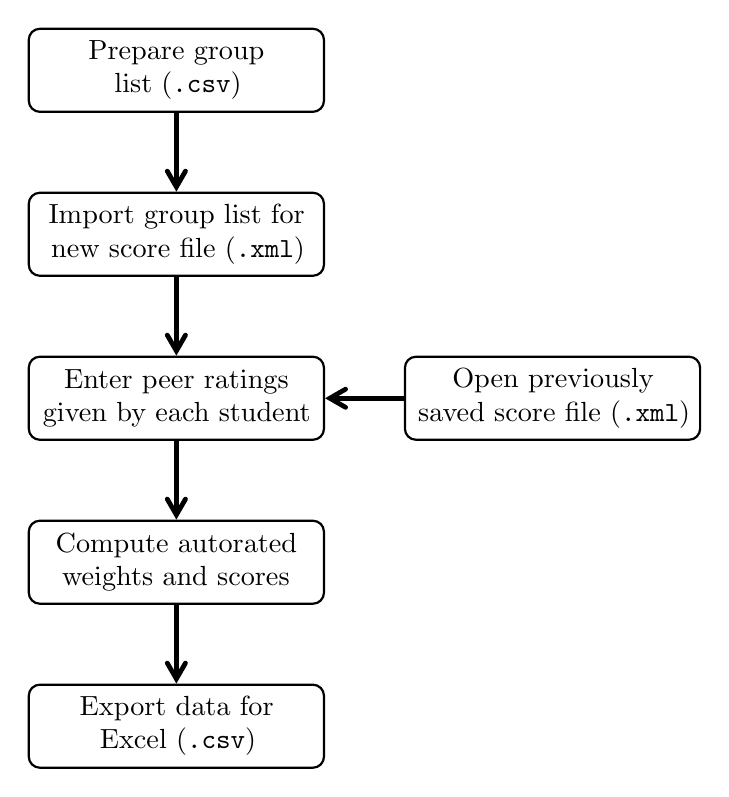
\begin{tikzpicture}
\tikzset{every node/.style={on chain,draw,thick,rounded corners,
minimum height=3em, text width=10em, align=center}}
\begin{scope}[start chain=going below]
\node (prepare-group) {Prepare group list (\texttt{.csv})};
\node (import-group) {Import group list for new score file (\texttt{.xml})};
\node (enter-rating) {Enter peer ratings given by each student};
\node (compute-score) {Compute autorated weights and scores};
\node (export-csv) {Export data for Excel (\texttt{.csv})};
\end{scope}
\node[right=of enter-rating] (open-score) {Open previously saved score file (\texttt{.xml})};

\path[draw,line width=0.4ex, ->,>= angle 60]
(prepare-group) edge (import-group) 
(import-group) edge (enter-rating)
(open-score) edge (enter-rating)
(enter-rating) edge (compute-score) 
(compute-score) edge (export-csv);
\end{tikzpicture}
\end{comment}

\bibliographystyle{plain}
\bibliography{refs}
\end{document}
